        \subsection{Monocromatizar Uno}
            \subsubsection{Implementación ANSI-C (SISD)}
                En esta implementacion se itera fila por fila, píxel por píxel, computando un píxel por iteración usando aritmética de enteros provista por C. El algoritmo es el mostrado por los docentes. Se obtienen los bytes de los correspondientes valores RGB, y se satura el resultado de la operacion (R + 2G + B) / 4 
            \subsubsection{Implementación ASSEMBLER (SIMD)}
                En nuestra implementación, calculamos de a 6 pixeles por iteracion. Para lograr esto, cargamos en los registros xmm0, xmm1, xmm2 y xmm3, las direcciones de forma tal que en el primer byte de cada registro, queden los valores B G G R de cada pixel respectivamente. Luego usamos la instrucción PSHUFB para reorganizar los registros como se ve en la imagen.
                
                \begin{figure}[htb]
                \begin{center}
                \leavevmode
                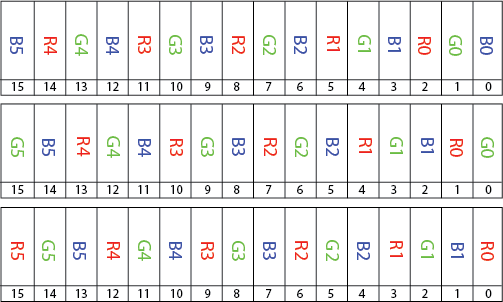
\includegraphics[width=0.5\textwidth]{carga_bytes_rgb.png}
                \end{center}
                \caption{Carga de bytes BGR}
                \end{figure}
                
                \begin{figure}[htb]
                \begin{center}
                \leavevmode
                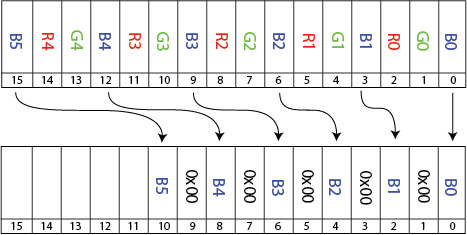
\includegraphics[width=0.5\textwidth]{gris_epsilon_uno_pshub.png}
                \end{center}
                \caption{pshufb para extender a dword}
                \end{figure}
                
                Luego de eso, nos quedan los registros con 6 words sin signo. Los sumamos, shifteamos usando la operación psraw 2 bits a la derecha cada word para dividir por 4. Hacemos un pack para pasar de words a bytes unsigned saturados. En xmm0 nos quedan los primeros 6 bytes con los valores de los píxeles finales. \newpage
                
                \begin{figure}[htb]
                \begin{center}
                \leavevmode
                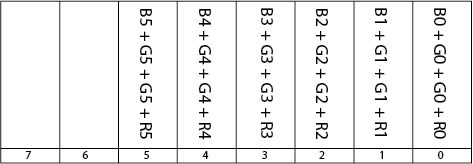
\includegraphics[width=0.5\textwidth]{gris_epsilon_uno_suma.png}
                \end{center}
                \caption{se suman los distintos colores}
                \end{figure}
                
                \begin{figure}[htb]
                \begin{center}
                \leavevmode
                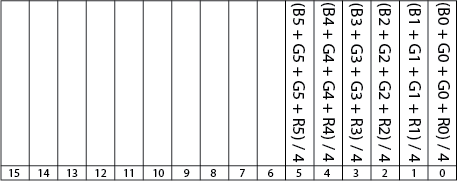
\includegraphics[width=0.5\textwidth]{gris_epsilon_uno_pack.png}
                \end{center}
                \caption{se transforman los resultados a bytes saturando}
                \end{figure}
                
                Finalmente, movemos los 64 bits más bajos de xmm0 a rax, y de ahí a memoria. Como solo tenemos 6 bytes en RAX que sirven, movemos EAX a memoria, shifteamos 32 bits a la derecha y movemos AX a memoria. Luego se pasa a la siguiente iteración.

        \subsubsection{Comparación de Performance (SISD vs SIMD)}

Acá va la comparación de performance entre C y ASM
